\documentclass[reprint,amsmath,amssymb,aps]{revtex4-2}


\usepackage{graphicx}
\usepackage{dcolumn}% Align table columns on decimal point
\usepackage{bm}
\usepackage{amsmath}
\usepackage{physics}
\usepackage{float}
\usepackage{hhline}

\hyphenchar\font=-1
%\usepackage{hyperref}% add hypertext capabilities
%\usepackage[mathlines]{lineno}% Enable numbering of text and display math
%\linenumbers\relax % Commence numbering lines

%\usepackage[showframe,%Uncomment any one of the following lines to test 
%%scale=0.7, marginratio={1:1, 2:3}, ignoreall,% default settings
%%text={7in,10in},centering,
%%margin=1.5in,
%%total={6.5in,8.75in}, top=1.2in, left=0.9in, includefoot,
%%height=10in,a5paper,hmargin={3cm,0.8in},
%]{geometry}

\begin{document}

\preprint{APS/123-QED}

\title{Campo Magnético da Terra}

\author{Amanda Schwartzmann}
\email{schwartzmann.a@ufabc.edu.br}
\author{Christian Noberto de Souza}
\email{christian.noberto@aluno.ufabc.edu.br}
\author{Deborah G. Fabri}
\author{Guilherme F. Evangelista}
\email{g.fortes@aluno.ufabc.edu.br}
\author{Henrique Dias Gomes}
\email{henrique.dias@aluno.ufabc.edu.br}
\affiliation{Universidade Federal do ABC}

\date{\today}

\begin{abstract}
Quando se sobrepõe o campo magnético da Terra a um outro campo conhecido, é possível obter a intensidade e direção do fluxo resultante e, assim, determinar a magnitude do campo terrestre. Neste trabalho, foram utilizadas bobinas de Helmholtz com um campo magnético uniforme para estimar a componente horizontal do campo terrestre. O coeficiente linear encontrado foi $c=(7,02 \pm 0,17).10^{-4}$ T/A ao variar a corrente na bobina e anotar o campo magnético correspondente na mesma, medido com um medidor de Tesla. O valor do campo terrestre horizontal rendeu um resultado de $^hB_E=(16,08\pm0,44)$ $\mu$T, com compatibilidade de até 4 desvios padrão da distribuição do valor esperado. Possíveis explicações para o alto desvio são a baixa exatidão dos equipamentos ou do modelo teórico para o cálculo do campo terrestre, além de influências externas como vento, movimento de pessoas, entre outros.

\textit{Relatório como parte avaliativa da disciplina \textbf{NHT3028 - Laboratório de Física II}, ministrada pelo Prof. Dr. Mauro R. Cosentino.}

\begin{description}
\item[Palavras chave]
\textit{Campo magnético da Terra}; \textit{Bobinas de Helmholtz};
\textit{Calibração}, \textit{Linhas isoclínicas\\ e linhas isógenas}.
\end{description}
\end{abstract}

%\keywords{Suggested keywords}%Use showkeys class option if keyword
                              %display desired
\maketitle

%\tableofcontents

\section{Introdução}

É sabido que a quantidade de radiação que chega até nós do espaço é amenizada devido a presença do campo magnético terrestre. É possível enxergar a existência da magnetosfera nas regiões sul e norte do nosso planeta, a partir das auroras boreais e austrais. Outro jeito de ver os efeitos do campo magnético da Terra é ao utilizar uma bússola, instrumento de navegação e orientação baseado na propriedade magnética que os materiais possuem, sendo utilizada desde o século XIII. 
Além de enxergar a existência do campo magnético terrestre por meio de seus efeitos, também é possível mensurá-lo por meio da sobreposição com um campo magnético conhecido, como será mostrado neste artigo.

\subsection{Fundamentos Teóricos}

Quando se sobrepõe o campo magnético da Terra a um campo magnético constante, cuja direção e intensidade são conhecidas, é possível determinar a magnitude do campo magnético terrestre devido à intensidade e direção do fluxo resultante. Para isso, pode-se colocar duas bobinas idênticas, distantes em um raio entre si (chamado de arranjo de Helmholtz), como visto na figura \ref{bobinas de helmholtz}.
\begin{figure}[h]
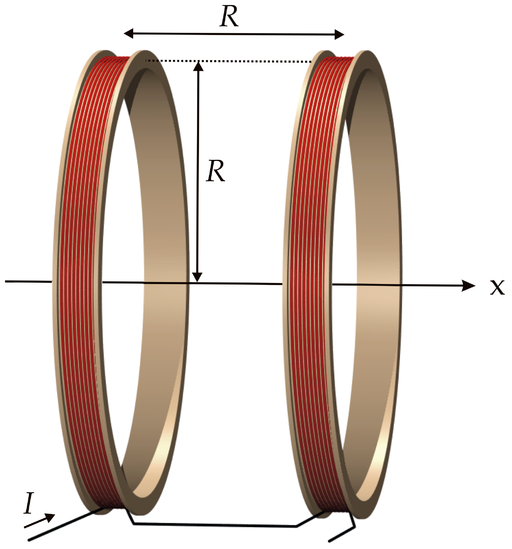
\includegraphics[scale=0.17]{Helmholtz_coils.png}
\caption{\label{bobinas de helmholtz} Arranjo de Helmholtz.}
\end{figure}

Nessa configuração, a primeira e a segunda derivada espacial da indução magnética no ponto central do arranjo se igualam a zero, assim nesse ponto o campo magnético é \cite{reitzfundamentos}
\begin{equation}
    ^\text{h}B_H =\frac{\mu_0 n I}{R} \qty(\frac{2}{\sqrt{5}})^3,
\end{equation}
com $n$ sendo o número de voltas na espira, $R$ o raio da bobina e $\mu_0$ a permeabilidade do vácuo. Assim, tendo $R=(0,1995\pm0,0005)$ m e $n=154$, tem-se que
\begin{equation}
    ^\text{h}B_H =cI,
\end{equation}
com $c=(6,94\pm0,02).10^{-4}$ T/A.
Deste modo, as bobinas de Helmholtz produzem um campo magnético relativamente uniforme em uma pequena região do espaço.

Nesse caso, há a sobreposição dos campos da bobina e da Terra. Pela lei dos senos, vale a seguinte relação para a componente horizontal do campo magnético da Terra $^hB_E$:
\begin{equation}
    \frac{\sin{\alpha}}{\sin(\varphi - \alpha)} = \frac{^\text{h} B_H}{^\text{h} B_E}.
\end{equation}

No caso em que o eixo da bobina é perpendicular ao da direção Norte-Sul ($\varphi \approx 90º$), a seguinte equação é aplicável para determinar o campo magnético da Terra:

\begin{equation}
    \tan(\alpha) = \frac{^\text{h}B_H}{^\text{h}B_E}
\end{equation}

\subsection{Objetivos}

O objetivo principal do experimento foi medir o campo magnético da Terra, e para isso foram necessárias duas tarefas.

A primeira tarefa consistiu na calibração do sistema, sendo preciso variar o valor da corrente ($I$) e medir o campo magnético ($^\text{h}B_H$) para cada valor de corrente, a fim de se extrair a constante da bobina através do coeficiente angular da reta ajustada para esses dados.

Assim sendo, após a calibração, a segunda tarefa consistiu em variar a corrente elétrica na bobina de forma que a agulha da bússola sofresse deflexões, dados estes coletados para que o cálculo do campo magnético terrestre seja realizado a partir do coeficiente angular do ajuste linear dos dados.

\section{Metodologia}

\subsection{Lista de Materiais}
Para a realização do experimento os materiais utilizados foram:
\begin{itemize}
    \item Bússola;
    \item Bobinas de Helmholtz com 154 espiras;
    \item Fontes de corrente contínua;
    \item Multímetros;
    \item Medidor de Tesla;
    \item Resistor variável (reostato).
\end{itemize}

As especificações dos materiais são:
\begin{enumerate}
    \item \textbf{Bússola}
    \begin{enumerate}
        \item Especificações Técnicas:
        \begin{itemize}
            \item Menor medida: 2 $^o$;
            \item Incerteza: 1 $^o$.
        \end{itemize}
    \end{enumerate}
    \item \textbf{Bobinas de Helmholtz}
    \begin{enumerate}
        \item Fabricante: Phywe Systeme \textregistered;
        \item Modelo: Par de bobinas de Helmholtz (Item no.: 06960-00); 
        \item Quantidade: 1 par;
        \item Especificações Técnicas \cite{bobinas}:
        \begin{itemize}
            \item Diâmetro da bobina: 400 mm;
            \item Número de espiras: 154;
            \item Corrente máxima por bobina (C.C.): 5 A;
            \item Resistência da bobina: 2.1 $\Omega$.
        \end{itemize}
    \end{enumerate}
    
   \item \textbf{Medidor de Tesla}
    \begin{enumerate}
        \item Fabricante: Phywe Systeme \textregistered;
        \item Modelo: 13610-90...93; 
        \item Quantidade: 1;
        \item Especificações Técnicas \cite{teslameter}:
        \begin{itemize}
            \item Temperatura de operação: 5 $^o$C - 40 $^o$C;
            \item Intervalo de medida: 10$^{-5}$ - 1999 mT;
            \item Incerteza para 0-20 mT: 0.01 mT.
        \end{itemize}
    \end{enumerate}
    
   \item \textbf{Fonte Universal}
    \begin{enumerate}
        \item Fabricante: Phywe Systeme \textregistered;
        \item Modelo: Fonte Universal (Item no.: 13500-90/-93); 
        \item Quantidade: 1;
        \item Especificações Técnicas \cite{fonteuniversal}:
        \begin{itemize}
            \item Tensão de saída: De 0.05 até 18 VDC;
            \item Corrente de saída: ajustável de 0.05 A até 5 A;
            \item Incerteza: 10 mV;
            \item Resistência interna: $20 \text{m}\Omega$.
        \end{itemize}
    \end{enumerate}
    
%    \item \textbf{Fonte Universal Variável}
 %   \begin{enumerate}
  %      \item Fabricante: Phywe Systeme %\textregistered;
  %      \item Modelo: Fonte Universal Variável (A.C. ou D.C) (Item no.: 13530-93); 
  %      \item Quantidade: 1;
   %     \item Especificações Técnicas \cite{fonteuniversalvar}:
    %    \begin{itemize}
     %       \item Tensão de saída: De 0 até 12 %VDC pulsante;
      %      \item Corrente de saída: 5 A;
       %     \item Frequência de saída: 100 Hz.
    %    \end{itemize}
%    \end{enumerate}

    \item \textbf{Multímetro de bancada digital}
    \begin{enumerate}
        \item Fabricante: Minipa \textregistered;
        \item Modelo: MDM-8045A; 
        \item Quantidade: 2;
        \item Especificações Técnicas \cite{multimetro}:
        \begin{itemize}
            \item Máxima corrente de entrada: 20 A por 15 segundos;
            \item Queda de tensão máxima: 200 mV
            \item Precisão na faixa de utilização:
        \item Precisão de (0,35\%+10D) na faixa de corrente trabalhada
        \end{itemize}
    \end{enumerate}
         \item \textbf{Reostato}
          \begin{enumerate}
        \item Fabricante:  Phywe Systeme \textregistered;
        \item Modelo: 06114-02 ; 
        \item Quantidade: 1;
        \item Especificações Técnicas \cite{reostato}:
        \begin{itemize}
            \item Capacidade de carga de 1,8 A;
            \item Resistência de 100 Ohm, $\pm$ 10\%
                    \end{itemize}
    \end{enumerate}
\end{enumerate}
       
Os materiais listados, com exceção dos multímetros, fazem parte do Kit de Experimentos para Física, feitos pela Phywe Systeme \textregistered.

\subsection{Montagem Experimental}
A montagem do experimento foi realizada de acordo com a figura \ref{pardebobinas}:

\begin{figure}[H]
\centering
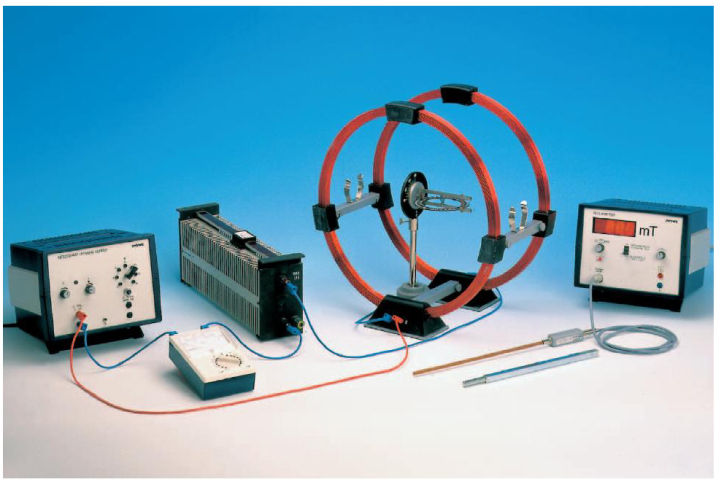
\includegraphics[scale=0.3]{aparato2.png}% Here is how to import EPS art
\caption{\label{pardebobinas} Aparato experimental ideal.}
\end{figure}

Inicialmente, o eixo das bobinas de Helmholtz foi alinhado com campo magnético terrestre, de forma que as linhas de campo da bobina fiquem perpendiculares à agulha da bússola. Esta foi posicionada no ponto central entre as duas bobinas conforme a figura \ref{aparato1}.
\begin{figure}[H]
\centering
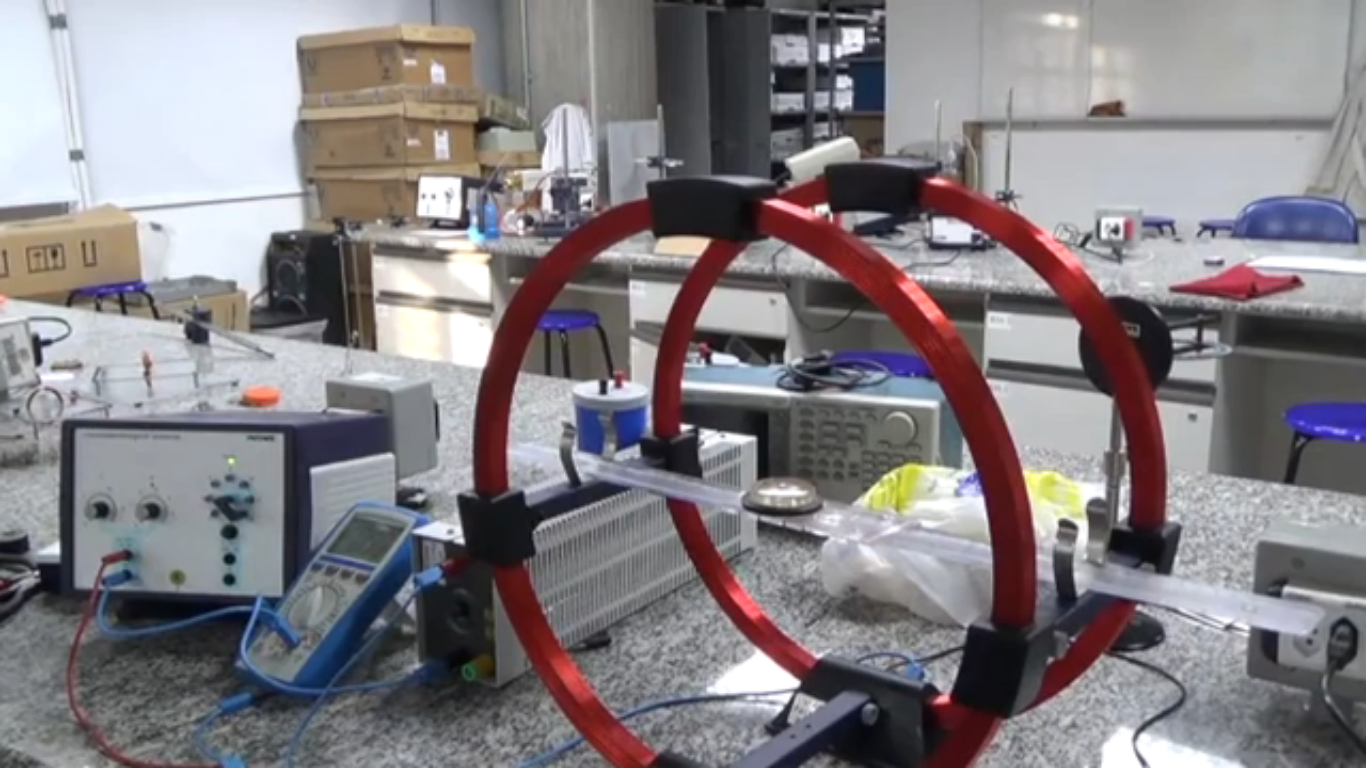
\includegraphics[scale=0.18]{aparato1.png}
\caption{\label{aparato1} Aparato experimental preparado para a coleta de dados \cite{earthmagfield}.}
\end{figure}

Em seguida a sonda Hall foi fixada no centro das bobinas de Helmholtz, a fim de determinar a curva de calibragem em função do campo magnético das bobinas e da corrente fornecida pela fonte.

Um esquema elétrico mais detalhado do circuito composto pelas bobinas de Helmholtz e o reostato pode ser observado na figura \ref{reostato}.
\begin{figure}[H]
\centering
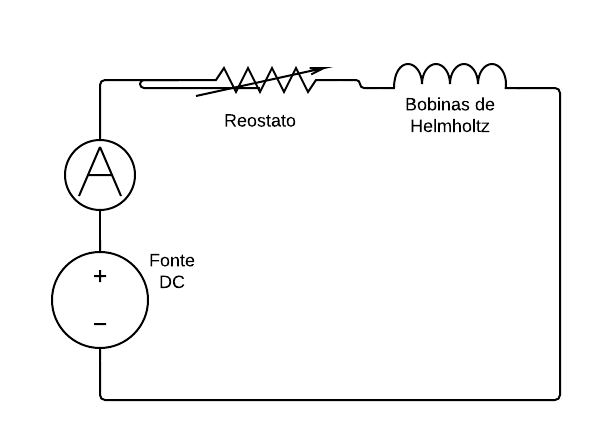
\includegraphics[scale=0.7]{reostato1.png}
\caption{\label{reostato} Diagrama elétrico da montagem adotada no experimento.}
\end{figure}

\subsection{Procedimento Experimental}

Como mencionado anteriormente, o procedimento experimental foi dividido em 2 tarefas, que serão descritas separadamente e de forma detalhada nesta seção.

\begin{enumerate}
    \item \textbf{Tarefa 1:} Foi construída uma curva de calibragem utilizando a sonda Hall fixada no centro das bobinas de Helmholtz. A componente horizontal da densidade de fluxo magnético do par de bobinas foi obtida pelo medidor de Tesla enquanto foi variado a intensidade da corrente aplicada nas
    bobinas (em uma faixa de 0 até 1,5 A), modificando tanto a posição do reostato como os valores nominais da fonte. Em seguida estes dados foram alocados na tabela \ref{tab:calibracao} e foi montado o gráfico apresentado na figura \ref{fig:calibracao}. De acordo com o coeficiente angular deste gráfico foi determinado o fator de calibração para que se possa iniciar as medidas da componente horizontal do campo terrestre.
    \item \textbf{Tarefa 2:} Foram calculados os valores do campo gerado pelas bobinas de Helmholtz $^\text{h}B_H$ considerando o fator de calibração $c$ para as diferentes intensidades da corrente aplicadas na tarefa 1 conforme a tabela \ref{tab:calibracao}. Para cada um dos valores de $^\text{h}B_H$ foi registrada a deflexão angular da bússola em relação à sua posição inicial $\alpha$, e os valores de $\tan(\alpha)$ foram registrados na tabela \ref{tab:medida}. Para essa etapa, foi estimado o valor da componente horizontal do campo magnético do planeta através da calculadora de campo magnético da \textit{National Centers for Environmental Information}\cite{efieldcalc}, calculada para a localização 'Avenida dos Estados, 5001, Santo André', com 760 m de altitude com relação ao nível do mar em 18/10/2019. Um \textit{print} das configurações é exibido na figura \ref{fig:efieldcalc}.
    \begin{figure}[H]
        \centering
        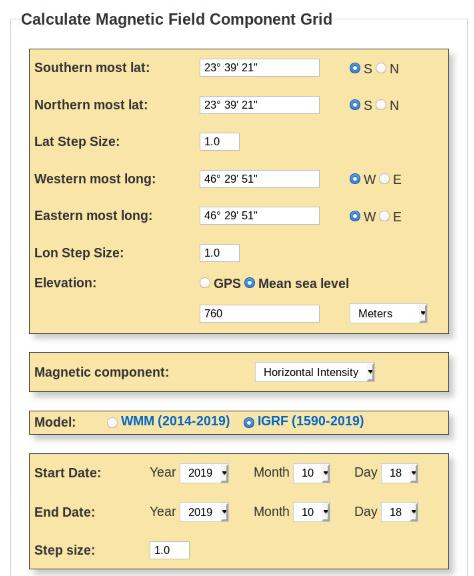
\includegraphics[scale=0.45]{CALCULADORA2.jpeg}
        \caption{Configuração para o cálculo da componente horizontal do campo magnético da Terra.}
        \label{fig:efieldcalc}
    \end{figure}
  
\end{enumerate}
 O valor divulgado pelo International Geomagnetic Reference Field (IGRF) é de (17,84 $\pm$ 0,13) $\mu$T. Segundo o  World Magnetic Model (WMM) também se obtém o mesmo valor.
 
\section{Apresentação de Dados e Análise de resultados}

\subsection{Calibração da bobina de Helmholtz}

Ao variar-se a intensidade da corrente aplicada na bobina, verificou-se valores crescentes do campo magnético correspondente, como observado na tabela \ref{tab:calibracao}.

\begin{table}[H]
\centering
\caption{\label{tab:calibracao} Valores da corrente na bobina e campo magnético correspondente.}
\begin{tabular}{cc}
\hhline{==}
$I$ (mA)            & $^\text{h}B_H$ (mT)              \\ \hline
0,070 $\pm$ 0,001 & 0,00   $\pm$ 0,01   \\
19,99 $\pm$ 0,07  & 0,04   $\pm$ 0,01   \\
39,4 $\pm$ 0,1    & 0,07   $\pm$ 0,01   \\
60,0 $\pm$ 0,2    & 0,09   $\pm$ 0,01   \\
80,2 $\pm$ 0,3    & 0,10   $\pm$ 0,01   \\
100,0 $\pm$ 0,4   & 0,11   $\pm$ 0,01   \\
119,9 $\pm$ 0,4   & 0,12   $\pm$ 0,01   \\
140,3 $\pm$ 0,5   & 0,13   $\pm$ 0,01   \\
196,7 $\pm$ 0,7   & 0,17   $\pm$ 0,01   \\
260,2 $\pm$ 0,9   & 0,22   $\pm$ 0,01   \\
318,6 $\pm$ 1,1   & 0,25   $\pm$ 0,01   \\
377,5 $\pm$ 1,3   & 0,30   $\pm$ 0,01   \\
439,5 $\pm$ 1,5   & 0,34   $\pm$ 0,01   \\
502,4 $\pm$ 1,8   & 0,38   $\pm$ 0,01   \\
\hhline{==}
\end{tabular}
\end{table}

Com estes valores, foi montado o gráfico \ref{fig:calibracao} utilizando o software \textit{QTIplot} 0.9.8.6, onde pode-se observar uma relação linear entre as duas grandezas. O ajuste linear teve como coeficiente da reta $c=(7,02 \pm 0,17).10^{-4}$ T/A, que pode ser comparado ao valor previsto pela teoria \cite{efieldcalc} calculando-se o erro normalizado $E_c$:
\begin{equation}
    E_c=\frac{|6,94-7,02|}{\sqrt{0,02^2+0,17^2}}=0,47,
\end{equation}
que demonstra uma medida compatível com o valor teórico para até um desvio padrão da distribuição.

\begin{figure}[H]
    \centering
    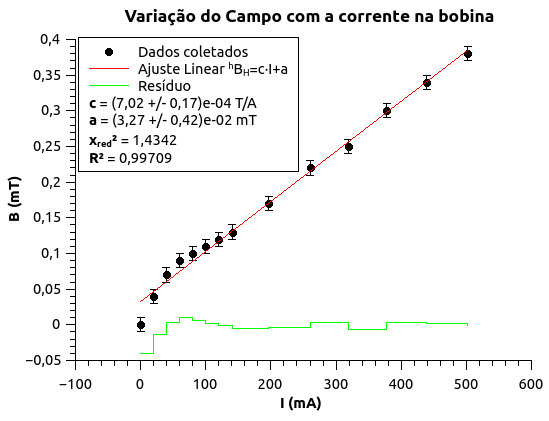
\includegraphics[scale=0.58]{Graph1.png}
    \caption{Relação entre a corrente na bobina e o campo magnético correspondente.}
    \label{fig:calibracao}
\end{figure}

É possível perceber na figura \ref{fig:calibracao} que o valor para $\chi_{red}^2$ é um pouco maior que um, indicando que o ajuste linear é compatível. Ainda é possível observar um valor próximo de $1$ para $R^2$, indicando uma boa correlação linear e um pequeno coeficiente linear $a$ em relação à ordem da amplitude da faixa de dados no eixo de $B$. Os resíduos mais altos para essa análise se encontram em valores menores de corrente, o que deve se justificar por uma alta oscilação relativa na fonte de corrente e nos valores indicados no medidor de Tesla.

\subsection{Medida da componente horizontal do campo magnético da Terra}

Os valores da tangente do ângulo de deflexão da bússola em função da variação da componente horizontal do campo magnético estão apresentados na tabela \ref{tab:medida}.

\begin{table}[H]
\centering
\caption{\label{tab:medida} Valores do campo magnético na bobina e ângulo de deflexão da bússola.}
\begin{tabular}{cc}
\hhline{==}
$^\text{h}B_H$ (10$^{-2}$ mT) & $\tan(\alpha)$ \\ \hline
0,000  $\pm$ 0,000   & 0,00   $\pm$ 0,02    \\
0,710  $\pm$ 0,002   & 0,49   $\pm$ 0,02    \\
1,410  $\pm$ 0,005   & 0,93   $\pm$ 0,03    \\
2,105  $\pm$ 0,007   & 1,33   $\pm$ 0,05    \\
2,802  $\pm$ 0,010   & 1,73   $\pm$ 0,07    \\
3,485  $\pm$ 0,012   & 2,05   $\pm$ 0,09    \\
4,208  $\pm$ 0,015   & 2,75   $\pm$ 0,15    \\
4,915  $\pm$ 0,017   & 3,08   $\pm$ 0,18    \\
5,620  $\pm$ 0,020   & 4,01   $\pm$ 0,30    \\
6,318  $\pm$ 0,022   & 4,70   $\pm$ 0,40    \\
7,042  $\pm$ 0,025   & 4,70   $\pm$ 0,40    \\
7,697  $\pm$ 0,027   & 5,14   $\pm$ 0,48    \\
\hhline{==}
\end{tabular}
\end{table}

Com os valores da tabela, foi montado o gráfico \ref{fig:medida}, que resulta em um coeficiente angular $^hB_E^{-1}=(62,2\pm1,7)$ mT$^{-1}$ e um valor para a componente horizontal do campo de $^hB_E=(16,08\pm0,44)$ $\mu$T. Assim, é possível fazer uma comparação com o valor esperado para o campo através do erro normalizado $E_B$:
\begin{equation}
    E_B=\frac{|17,84-16,08|}{\sqrt{0,13^2+0,44^2}}=3,84,
\end{equation}
ou seja, a medida só pode ser considerada compatível em 3,84 desvios padrão da distribuição. 

\begin{figure}[H]
    \centering
    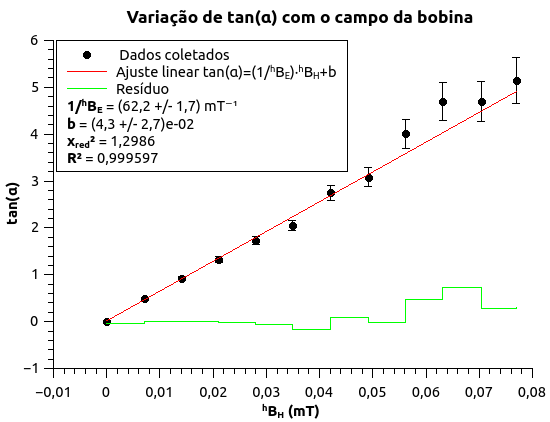
\includegraphics[scale=0.58]{Graph2.png}
    \caption{Relação entre o campo magnético na bobina e ângulo de deflexão da bússola.}
    \label{fig:medida}
\end{figure}

No gráfico, há um valor do coeficiente linear pequeno em relação à ordem de grandeza da $\tan(\alpha)$. O ajuste ainda apresenta um valor de $\chi_{red}^2$ bem próximo da unidade indicando um bom ajuste, assim como $R^2$, que indica uma boa correlação e comportamento linear dos dados. O gráfico dos resíduos mostra que há um maior erro para altos valores de campo magnético na bobina, o que experimentalmente é justificado pois torna-se mais difícil ter precisão para coletar os dados da bússola devido à alta sensibilidade.

\section{Conclusão}

Com os resultados apresentados, é possível concluir que a medida da componente horizontal teve um alto desvio em sua exatidão em relação à sua precisão. Uma possível explicação é que o modelo teórico utilizado para calcular a componente do campo não é perfeito e pode apresentar algumas falhas, além das medidas terem sido realizadas com equipamentos que poderiam ser mais sofisticados e que levariam a um valor mais próximo do intervalo de compatibilidade. De todo modo, a ordem de grandeza da componente pôde ser verificada com um bom valor estimado.


Um tratamento da componente vertical do campo pode ser realizado a fim de testar a compatibilidade entre resultados do experimento e do modelo, esclarecendo melhor o estudo realizado.

\newpage

\nocite{*}

\bibliography{apssamp.bib}

\end{document}